%%% template.tex
%%%
%%% This LaTeX source document can be used as the basis for your technical
%%% paper or abstract.

%%% The parameter to the ``documentclass'' command is very important.
%%% - use ``review'' for content submitted for review.
%%% - use ``preprint'' for accepted content you are making available.
%%% - use ``tog'' for technical papers accepted to the TOG journal and
%%%   for presentation at the SIGGRAPH or SIGGRAPH Asia conference.
%%% - use ``conference'' for final content accepted to a sponsored event
%%%   (hint: If you don't know, you should use ``conference.'')

\documentclass[tog]{acmsiggraph}
\usepackage{mathtools}
\usepackage[utf8]{inputenc}
\usepackage{float}
\usepackage{url}
\usepackage{amssymb}

%%% Make the ``BibTeX'' word pretty...

\def\BibTeX{{\rm B\kern-.05em{\sc i\kern-.025em b}\kern-.08em
    T\kern-.1667em\lower.7ex\hbox{E}\kern-.125emX}}

%%% Used by the ``review'' variation; the online ID will be printed on 
%%% every page of the content.

\TOGonlineid{45678}

%%% Used by the ``preprint'' variation.

\TOGvolume{0}
\TOGnumber{0}

\title{A Simplified Contact Model for Treating the Balance of Biped Virtual Characters}

\author{Danilo Borges da Silva\thanks{e-mail:danilobs@lia.ufc.br}\\UFC}
\pdfauthor{Danilo B. da Silva}

%3D interaction; Virtual humans and avatars; Physics-based animation; Controllers;
\keywords{3D interaction, virtual humans and avatars, physics-based animation, controllers}

\begin{document}

%%% This is the ``teaser'' command, which puts an figure, centered, below 
%%% the title and author information, and above the body of the content.

%---------------------- Imagem horizontal
 %\teaser{
 %  \includegraphics[height=1.5in]{images/sampleteaser}
 %  \caption{Spring Training 2009, Peoria, AZ.}
 %}

\maketitle

\begin{abstract}

In this work, we present a physically-based model for maintaining the equilibrium of biped characters. We use Proportional-Derivative (PD)
Controllers to mimic the characteristics of angular joints, and deal with the equilibrium through a method that uses the transpose of the 
Jacobian matrix that relates the angular and linear momentum at the Center of Mass (COM) of the character’s body to the corresponding quantities
at all its members, which are treated as end effectors.
%Namely, all links work together, as a whole, in order to balance the character.
Namely, the balance control involves all links, as a whole, and not only the lower body.
Also, we propose a simple contact model for treating the interaction between
the feet and the ground that confers great stability to the character and makes it easier for the controller and for the starting of the 
simulation. It also makes it convenient for the animator to adjust the model so as to consider a trade-off between more physical realism and 
more stability. The system does not use optimization and is simple to implement. Unlike existing methods for control based on reference motions, our framework 
does not require preprocessing of the reference motion, nor does it rely on inverse dynamics or optimization methods.
The robustness of the controller is demonstrated through a 
series of tests that show that the character is able to adapt its posture and maintain equilibrium either under the influence of external actions
from the environment or when it follows unaltered reference motions. 

%This work presents a model for controlling physics-based bipeds
% characters in a simulated environment with treatment of balance. Controllers Proportional-Derivative (PD) are used
%to mimic angular characteristics of the joints, with specific form of Jacobian Transpose for balance control.
%The Jacobian is constructed based on linear and angular momenta of the character related to the Center of Mass (COM) of the character, 
%allowing control of balance involves all its parts, as a whole, not just your legs.
%A proposed model of contact gives the character enough stability, facilitating the work of the controller and allows easy initialization of the simulation.
%Also, if prefer, is allowed to animator sacrifice a little of physical correctness of simulation in exchange for greater stability,
%which consists of a very useful tool in practice.
%The system does not require optimization and is simple to implement.
%The robustness of the controller is demonstrated by a variety of tests, in which the character can be capable 
%so much adapt to the environment external interventions like mimic movements captured used directly without preprocessing.

\end{abstract}

%\begin{CRcatlist}
%  \CRcat{I.3.3}{Computer Graphics}{Three-Dimensional Graphics and Realism}{Display Algorithms}
%  \CRcat{I.3.7}{Computer Graphics}{Three-Dimensional Graphics and Realism}{Radiosity};
%\end{CRcatlist}

\keywordlist

%% Required for all content. 

\copyrightspace

\section{Introduction}

In the field of physics-based control of human motion, a simulated character usually consists of a structure of articulated rigid bodies (links)
with internal angular actuators located at the joints. The feet are usually represented in a very simplified way, through boxes (parallelepipeds),
and, for that reason, the interaction with the ground is very discontinuous \cite{bib:Lee10,bib:Jain11}. That type of model (articulated rigid
links and simplified rigid feet plus angular actuators), however, is capable of capturing the fundamental aspects of the human musculoskeletal
system. Therefore, researchers were able to develop successfully a number of controllers for performing multiple tasks involving balance \cite{bib:Geijtenbeek13}. 
Despite the remarkable achievements, the simplified model still imposes a constraint that prevents the virtual human from exhibiting the same
abilities of a real human. Thus, more robust models have been proposed recently \cite{bib:Jain11,bib:Wang12}.

\begin{figure}[thbp]
\centering
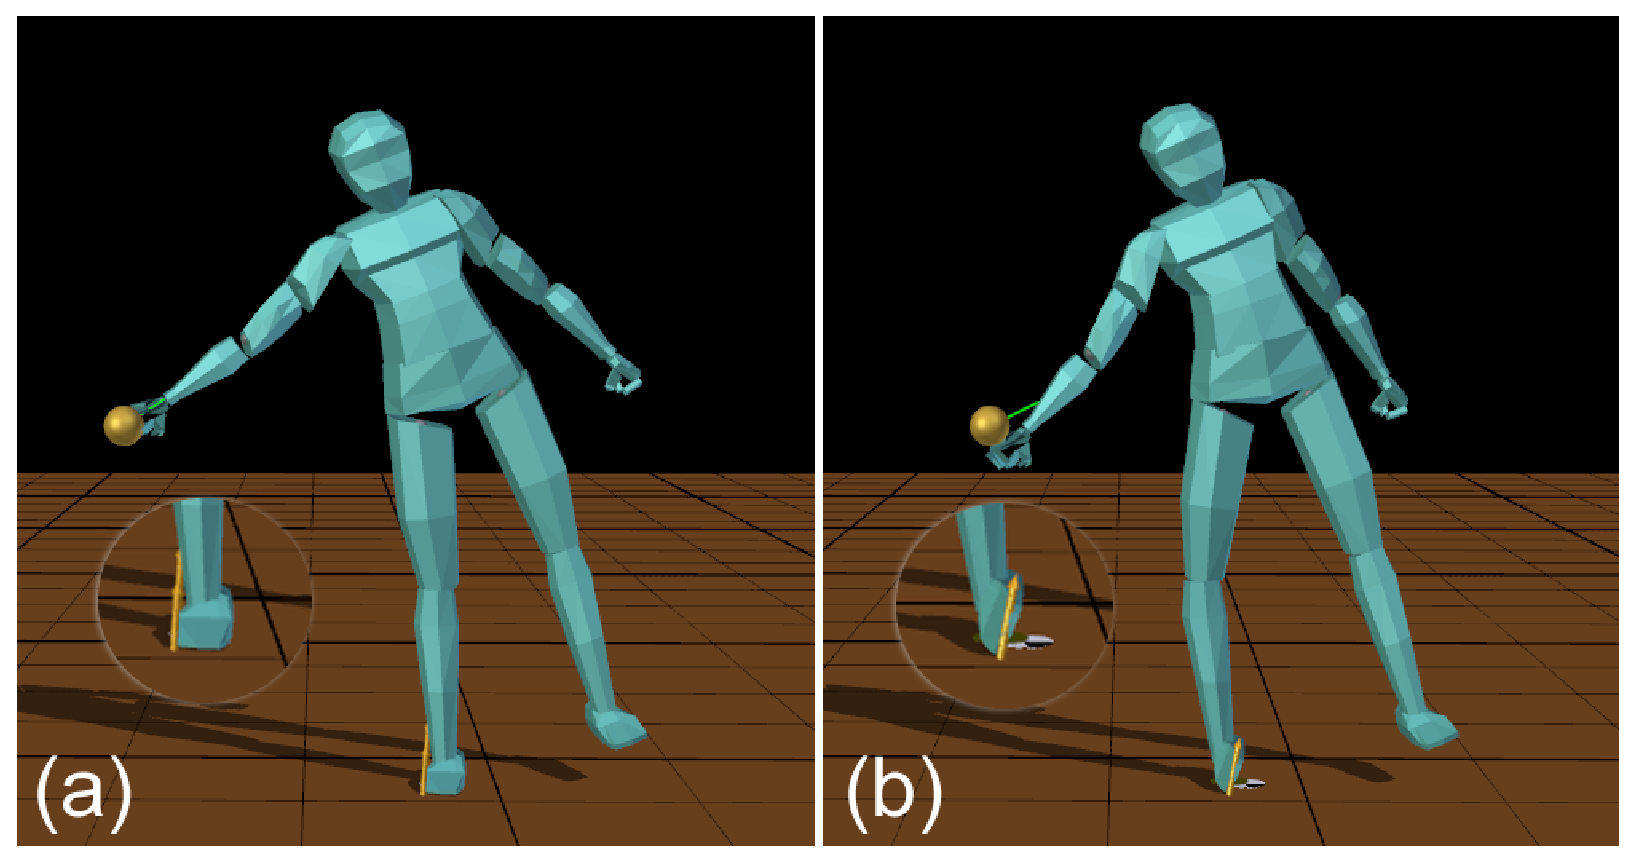
\includegraphics[width=9cm]{images/PefirmeXPedeslizando.eps}
\caption{The stance foot contact model. (a) The proposed simplified contact model increases the stability between the foot and the ground, 
         allowing the stance foot remains steady, even when the used geometry in the simulation is not appropriate.
         (b) Without the proposed model, the internal torque applied to the foot is not compensated. In this case, more complex controllers, involving optimization
         \protect\cite{bib:Macchietto09,bib:Geijtenbeek12}, would be required.}
\label{fig:PefirmeXPedeslizando}
\end{figure}



The balance of a virtual character at a given instant depends upon the complex interrelation between the set of external forces and the set
of internal forces produced by the actuators, which are located at the joints, and that reconfigure each individual rigid link of the articulated
structure, altering the overall posture’s configuration. The dynamic reconfiguration of the posture modifies the external contact forces 
continuously. Thus, if the only parts of the body in contact with the ground are the feet, the way each individual foot is modeled will 
have a strong influence on the overall distribution of the external contact forces, and, therefore, on the balance of the character. Because a 
real foot is structurally complex and flexible, it can generate an infinite number of external contact forces redistributions when trying to 
maintain the global equilibrium. The feet models used for simulations are much less complex and, therefore, cannot reproduce the same 
redistribution of contact forces obtained with real feet. Jain and Liu \shortcite{bib:Jain11} have shown that, when the complexity of the foot model
increases, an existing controller becomes more robust because it is able to represent the distribution of contact forces better.


In this work, we argue that the use of a stable contact model facilitates the design of robust controllers, without the need of a sophisticated
model for the foot of the virtual human. We believe that modeling a realistic foot that offers the same range of redistribution of contact forces
that a real foot offers is important. However, that still requires a great research effort \cite{bib:Jain11}. Therefore, in a simulation, we 
propose to uncouple the foot’s model from the foot’s physical interaction with the ground.


Regarding two extreme situations, in which the friction between the foot and the ground is either infinite or zero (or buried foot vs. wooden leg),
is easy to see that the more
firmly the foot is on the ground, the more control over the global equilibrium the character will have. From the point of view of a physical
simulation, keeping the foot firmly on the ground implies a null resultant torque. Therefore, since an instantaneous equilibrium condition 
implies not only global equilibrium, but also the equilibrium of each individual link of the character’s structure, the forces acting on the foot 
must be also in equilibrium. So, what we seek is to maintain the equilibrium between the ground forces acting on the foot with the internal
forces transmitted by the actuators connected to the foot. This is a control problem because those forces are constantly being updated. Figure 
\ref{fig:PefirmeXPedeslizando} illustrates what happens when the torque applied to the foot by the actuators is not in equilibrium with that
produced by the Ground Reaction Forces (GRFs).

What is proposed in this work is to produce, artificially, the torques that would be provided by the ground forces generated by the accommodation
of a complex foot with the ground. Those artificial torques are generated independently of the foot model used, and, therefore, simplify the 
control of the foot vs. ground interaction. However, although the artificial torques are not compatible with the foot’s geometry indeed used in 
the simulation, they have plausible values, and still can be considered physically correct, validating the generated motion. The main advantages
of this approach are its simplicity and its independence from a sophisticated foot model.

It is obvious that, if no bounds are imposed to the artificially generated torques, the physical realism may be lost and the character would be 
endowed with superpowers. However, sacrificing the motion’s physical correctness in order to gain stability may be desirable in some situations. 
The proposed technique explores that flexibility of controlling stability in order to provide a robust tool that gives more freedom to the 
animator.

The Jacobian matrix of the mapping between two coordinate systems has been used as an abstraction layer to simplify the control of balance
\cite{bib:Coros10,bib:GeijtenbeekState12,bib:Geijtenbeek12}. That abstraction allows the center of mass (COM) of the character
to be controlled directly through the application of virtual forces and torques to the COM. Those virtual forces and torques are, in fact,
converted to equivalent internal torques that are applied to the joints by the actuators. Most of the works in the literature do not consider
the influence of the upper part of the character in the construction of the Jacobian. In this paper, however, we present a construction based
on the total momentum of the character at its COM, allowing the control of balance to involve the character as a whole, and not only its 
lower limbs.

\section{Related Work}

%Tentar manter esta seção resumida de modo que o artigo se mantenha com 8 páginas

%--------------Incluir esses parágrafos (pode resumí-los, caso necessário)-------------------

In this section, we present the most relevant works and discuss some of their differences with respect to the current work. Two main aspects
are considered in the discussion: the modeling of the foot and the way the Jacobian matrices are used for stability control.


  %----------Comparar com os seguintes artigos--------------

    %\cite{bib:Jain11,bib:Geijtenbeek12,bib:Wrotek06,bib:Witkin88} %mais importante
      %Jain11: abordagem divergente da nossa ideia (eles propõem melhorar a modelagem do pé, enquanto nós propomos desacoplar modelagem do pé e sua interação com o chão)
      %Geijtenbeek12: parecido em muitos pontos (mas não usamos otimização)
      %Wrotek06: ideia de aplicar torques externos (eles aplicam explicitamente, nós aplicamos sutilmente e ainda usando argumentos que validam o movimento gerado sob certas condições)
        %validar movimento = corretude física
      %Witkin88 + spacetime constraints papers: spacetime constraints já tratam geometria do pé e interação com o chão independentemente (nós trazemos essa ideia para simulação)
        %eles consideram GRFs como parte dos parâmetros a serem obtidos por otimização, %o que garante a corretude física dessas GRFs? o movimento gerado pode ser dito fisicamente correto?
        %as quais são validadas fisicamente apenas através de restrições usadas no problema de otimização, baseadas no cone de fricção

    %\cite{bib:Zordan02,bib:Yin07,bib:Coros10} %menos importante

  %---------------------------------------------------------

Some authors argue that, in order to achieve greater stability of locomotion, the model of the character’s foot should reproduce as close as
possible the behavior of a real human foot. Wang et al.  \shortcite{bib:Wang09} increased the number of joints to model a more 
flexible foot that essentially consists of a greater number of rigid links. Jain and Liu \shortcite{bib:Jain11} modeled the foot as a
deformable object in order to test the hypothesis that ``ignoring the effect of deformable bodies at the site of contact negatively affects
the control algorithms, leading to less robust and unnatural character motions.''
Geijtenbeek et al. \shortcite{bib:Geijtenbeek12}, in turn, seem to have needed to use a foot with larger proportions, in order to increase the contact area with the ground and, thus, facilitate the achievement of successful results.

Considering the works that use Jacobian matrices for stability control, Coros et al. \shortcite{bib:Coros10} incorporate a form of
Jacobian transpose \cite{bib:Sunada94} to motion control resulting in versatile and generic actions for bipedal locomotion. That control method
is based on the control system of Pratt et al. \shortcite{bib:Pratt01}, which use virtual actuators. That same system is used as a basis to provide
balance to biped characters in ~\cite{bib:Geijtenbeek12,bib:Zordan02}. Regarding the construction of the Jacobian, the global DOFs of the
character (not actuated) should not be restricted to those related to the character’s global position only.  Thus, unlike the work of Coros et al.
\shortcite{bib:Coros10}, it is interesting that the character’s global orientation is also considered in the construction
of the Jacobian, allowing the application, at the COM, of virtual forces as well as of virtual torques. This paper considers global orientations
and positions in a unified way. Geijtenbeek et al. \shortcite{bib:Geijtenbeek12} also use global orientations and positions, but not in a unified manner.

While some authors \cite{bib:Abe07,bib:Macchietto09,bib:Wang09,bib:Geijtenbeek12} need to use optimization, even if offline, 
in order for their equilibrium strategies to work well, our contact model provides a stable and easily adjustable alternative for the treatment
of balance without optimization. Also, while Coros et al. \shortcite{bib:Coros10} use pose control graphs \cite{bib:Yin07} to 
design the style of the motion generated by the controller, the model proposed in this work allows that unaltered captured motions be used for
this purpose. The work of Geijtenbeek and his co-workers \cite{bib:Geijtenbeek12} also presents that functionality, but it requires optimization.

%--------------------------------------------------------------------------------------------

\section{Overview}

%Visao geral
\begin{figure*}[tbh]
     \centering
     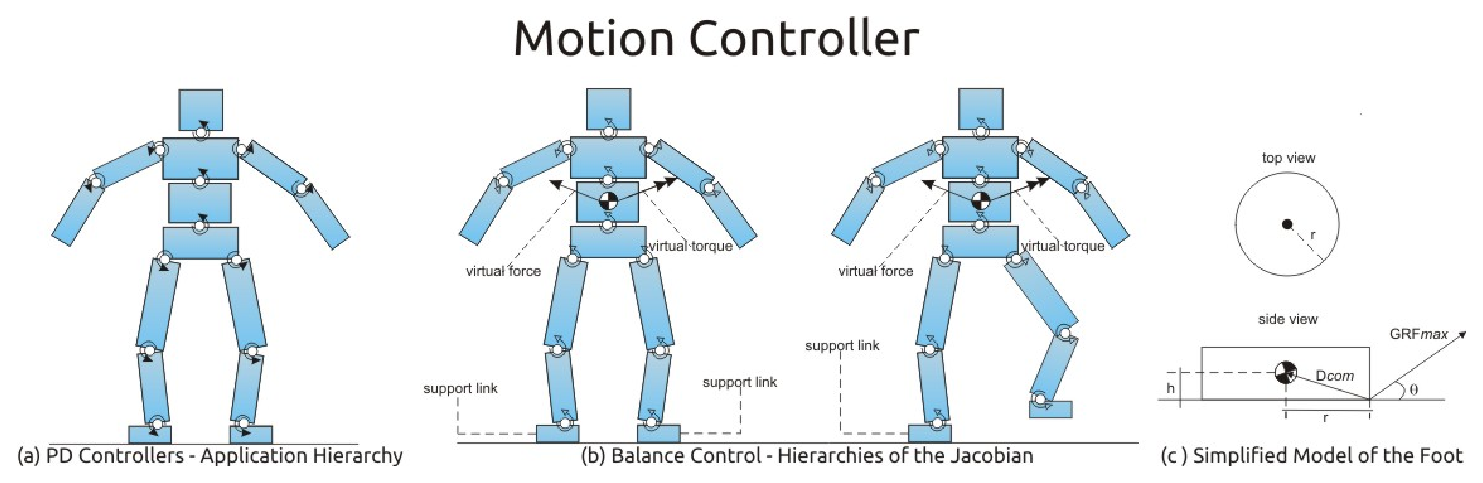
\includegraphics[width=18.4cm]{images/visaogeral-translate.eps} %height=5cm,
     \caption{Motion controller overview. (a) PD controllers are used to mimic the angular characteristics extracted from reference motions or specified by
the animator. (b) The Balance Control of the character uses a Jacobian transpose to compute the internal torques to be applied at its joints,
according to the hierarchy defined by the link that is in contact on the ground, from the virtual force and virtual torque applied at its center of mass. (c) The simplified
contact gives to the character greater stability, compensating part or the whole impact of its foot against the ground.}
     \label{fig:visaogeral}
\end{figure*}

As illustrated in Figure \ref{fig:visaogeral}, the structure of the proposed controller has three main components: PD Controllers, Balance Control
and Simplified Contact Model of the feet with the ground.


The PD controllers guarantee that the poses provided either by the user or by motion capture are achieved. In order to do that, they apply torques
to the joints according to a hierarchy that considers the pelvis as its root. However, PD controllers do not control the global DOFs directly. 
In fact, those DOFs are controlled by means of virtual forces and torques that are applied to the character’s COM.


The balance control component is responsible for computing those virtual forces and torques and converting them into equivalent internal torques,
through the transpose of the Jacobian matrix. The Jacobian matrix is assembled according to a hierarchy that considers the support foot as its 
root. Note that, in some situations, both feet may be considered simultaneously as the support.

Finally, the torque (or a fraction of it) applied to the support foot is artificially compensated in order to increase the stability of 
interaction with the ground and thereby facilitate the control of balance. Each one of the controller’s components is discussed in more 
detail in the following sections.

%%%%%%%%%%%%%%%%%%%%%%%%%%%%%%%%%%%%%%%%%%%%%%%%%%%%%

\section{PD Controllers}

The implementation of the PD controllers is based on \cite{bib:NunesTese12}, in which quaternions are used to represent the 3D orientations. 
Considering only spherical joints, each torque applied to a joint, $j$, is given by:

%
\begin{equation}
 ^{j}\tau_{pd} = k_{s}(q_{d}  q_{a}^{-1}) + k_{d}(\omega_{d} -\omega_{a}),
 \label{eq:toquepd3d}
\end{equation}
%
\noindent 
where $q_{a}$ and $q_{d}$ are, respectively, the current and the desired quaternions of the joint, $\omega_{a}$ and $\omega_{d}$ are the current 
and desired angular velocities of the joint, and $k_{s}$ and $k_{d}$ are user-defined constants. The expression  $q_{d}  q_{a}^{-1}$ corresponds to the 
three-dimensional version of the following two-dimensional angular difference ($\theta_d - \theta_a$). Note that the resulting quaternion still
needs to be converted to the axis and angle representation. The desired information can be obtained directly from captured motions, without any
adjustment. In contrast, some works require large adjustments \cite{bib:Yin07}. According to a pre-established hierarchy, applying a torque $\tau$ to a joint corresponds
to applying the same torque $\tau$ to its child link and the opposite torque -$\tau$ to its parent link.


%%%%%%%%%%%%%%%%%%%%%%%%%%%%%%%%%%%%%%%%%%%%%%%%%%%%%

%------traducao (tradutor 2) ok---------

\section{Balance Control}

As already stated, the balance control is required because the character's global DOFs do not have direct actuators.
Shortly, a Jacobian matrix is used to convert virtual forces and torques, to be applied to the COM, in equivalent internal joint torques.
This section is divided into three main parts: construction of the Jacobian matrix, calculation of the virtual force and
calculation of the virtual torque.

%-----------------------------------------------

\subsection{Jacobian's Construction}\label{subsec:Jacobiana}

The Jacobian matrix describes the linear relationship between the velocity of a specific point (end effector) and the velocities of the
joints which influence that point, according to a predefined hierarchy. Note the Jacobian involves only a sub-chain of articulated links,
starting from a fixed base (e.g. stance foot). To treat the balance, the COM of the character is usually chosen as the end effector.
Using the \textit{spatial vector notation} (Appendix \ref{ap:notacao6D}), we want to determine the Jacobian $J_ {com}$:
%
\begin{equation}
 ^{com}\phi_{com} = J_{com} ~ ^{J}\Phi_{J}
\label{eq:jacob}
\end{equation}
%
where $^b\phi_a$ represents the \textit{spatial velocity} of $a$ with respect to the frame $b$ (i.e., in the coordinates of $b$), and $^{J}\Phi_{J}$ corresponds to the vector formed by all joints' \textit{spatial velocities} together, in each joint's local coordinates.
Considering the character has $n$ joints in total,
$^{J}\Phi_{J} = \left( ^{j_{0}}\phi_{j_{0}}^T ~ ^{j_{1}}\phi_{j_{1}}^T ~ ... ~ ^{j_{n-1}}\phi_{j_{n-1}}^T \right)^T$ has dimension $6n\times1$.

However, considering the COM as a simple end effector means assuming that only some joints influence it, what clearly is not true.
In this work, all links are considered as end effectors, each having an exclusive Jacobian.
The velocities of all links, as well as their individual Jacobians, are then proportionally combined, according to their masses,
in order to calculate the character's total momentum, relative to its COM:
%
\begin{equation}
 \prescript{com}{}{ \left(\begin{array}{c} L \\ P \end{array}\right)_{c}} = \prescript{com}{}{ \left(\begin{array}{c} \mathcal{I} \cdot \omega \\ m \cdot v \end{array}\right)_{c}}
                                                                          = (\prescript{com}{c}{M}) (^{com}\phi _{com}),
\label{eq:MomTotal}
\end{equation}
%
%onde $L_p$ corresponde ao \emph{momentum} angular e $P_p$ ao \emph{momentum} linear do personagem, $\mathcal{I}_p$ corresponde à matriz de inércia total do personagem, relativa ao seu COM,
%e $m_p$ corresponde à massa total do personagem. $\prescript{com}{p}{M}$ é a \emph{massa 6D} total do personagem, em coordenadas do seu COM.
where $L$ corresponds to angular momentum, $P$, to linear momentum, $\mathcal{I}$, to inertia matrix,
$\omega$, to angular velocity, $m$, to mass, and $v$, to linear velocity.
The $c$ index encompasses the total information of the character. $\prescript{com}{c}{M}$
is the total \textit{spatial mass} of the character, in the coordinates of its COM.

The total momentum can also be obtained by the sum involving all links:
%
\begin{equation}
 \prescript{com}{}{ \left(\begin{array}{c} L \\ P \end{array}\right)_{c}} = \sum_l (\prescript{com}{l}{M})(^{com}\phi_{l})
                                                                          = \sum_l (\prescript{l}{com}{Ad})^{T} (^{l}_{l}M)(^{l}\phi_{l}),
\label{eq:MomSom}
\end{equation}
%
%onde o somatório em $l$ inclui todos os \emph{links} do personagem,
where the adjoint matrix $(\prescript{l}{com}{Ad})^{T}$ transforms the spatial momentum of each link $l$, given in local coordinates, in the coordinates 
of the COM. Note that spatial momentum, as well as \textit{spatial force}, is transformed with the inverse transpose of the adjoint matrix.

As mentioned, each link $l$ has an exclusive Jacobian, $J_{l}$, which relates your \textit{spatial velocity}, $^{l}\phi_{l}$, with the vector $^{J}\Phi_{J}$. 
Note that, according to a particular hierarchy, $^{l}\phi_{l}$ can be obtained by the sum of the \textit{spatial velocities} of all joints influencing the link $l$:
%
\begin{equation}
 ^{l}\phi_{l} = \sum_j {^{l}\phi_{j}} = \sum_j {^{l}_{j}Ad} ~ {^{j}\phi_{j}} = J_{l} ~ ^{J}\Phi_{J},
\label{eq:jacobIndividual}
\end{equation}
%
where the sum in $j$ includes all joints that influence the link $l$. Note that, in order to isolate the whole vector $^{J}\Phi_{J}$ at right, %detach/segregate %entire
that sum in $j$ could be replaced by the multiplication of $J_{l}$ and $^{J}\Phi_{J}$. Therefore, $J_ {l}$ corresponds to a matrix, with dimension $6\times6n$,
containing those adjoint matrices horizontally arranged at the locations corresponding to their respective joints, included in the sum. %summation.
%
Zero matrices with dimension $6\times6$ are placed at the locations corresponding to the joints that do not influence the link $l$.
%
For clarity, consider hypothetically that the character has only 6 joints. Also consider that, according to the adopted hierarchy, a link $l$
is influenced by the joints $j_{1}$, $j_{2}$ and $j_{4}$. The individual Jacobian of that link $l$ is defined as follows:
%
\begin{equation}
 ^{l}\phi_{l} = J_{l} ~ ^{J}\Phi_{J} = \left[ \begin{array}{cccccc} 0 & _{ j_{1} }^{l}Ad & _{ j_{2} }^{l}Ad & 0 & _{ j_{4} }^{l}Ad & 0
                                              \end{array} \right] ~ ^{J}\Phi_{J}.
\end{equation}

In order to facilitate the implementation, a given hierarchy may be represented by a table relating all joints (lines) to all links (columns) of the 
character. Each cell of that table is filled with 0 (zero) or 1 (one), according to the hierarchy. Filling a cell with 1 means that the joint
corresponding to that line influences the link corresponding to that column. Otherwise, the cell should be filled with 0. At each step of 
the simulation, both the hierarchy of the character and the Jacobians are updated according to the contacts between the feet and the ground.

Finally, combining the Equations \ref{eq:MomTotal}, \ref{eq:MomSom} and \ref{eq:jacobIndividual}, and comparing with the Equation \ref{eq:jacob},
we figure out the final expression of the Jacobian $J_{com}$,
%Note que essa \emph{Jacobiana espacial 6D baseada em momento}, $J$, é mais geral, descrevendo um relacionamento linear entre a \emph{velocidade 6D} relativa ao COM do personagem
%e as \emph{velocidades 6D} de \textbf{todas} as suas juntas.
which involves all joints of the character, and not only the lower limbs:
%
\begin{equation}
 J_{com} = (\prescript{com}{c}{M})^{-1} \sum_l (\prescript{l}{com}{Ad})^{T} (_{l}^{l}M) J_{l},
\end{equation}
%
where:
%
\begin{equation}
 \prescript{com}{c}{M} = \sum_l (\prescript{l}{com}{Ad})^{T} (_{l}^{l}M) (\prescript{l}{com}{Ad}).
\end{equation}
%

The operation $(\prescript{l}{com}{Ad})^{T} (_{l}^{l}M) (\prescript{l}{com}{Ad})$ transforms the \textit{spatial mass} matrix of each
link $l$, given in local coordinates, in the coordinates of the COM \cite{bib:NunesTese12}.

The internal \textit{spatial forces}, to be applied to the joints of the character, are obtained by the transpose of the Jacobian $J_{com}$, according to
the virtual \textit{spatial force}, composed by the concatenation of the virtual torque and the virtual force (Subsections \ref{torquevirtual} and \ref{forcavirtual}):
%
\begin{equation}
 ^{J}W_{J} = (J_{com})^T ~ ^{com}w_{com},
\label{eq:jacobTransp}
\end{equation}
%
where $^b{w}_a$ is the \textit{spatial force} of $a$ in the coordinates of $b$, and $^{J}W_{J}$ corresponds to the vector formed by all joints'
\textit{spatial forces} together, in each joint's local coordinates.
Similar to $^{J}\Phi_{J}$ (Equation \ref{eq:jacob}), $^{J}W_{J} = \left( ^{j_{0}}w_{j_{0}}^T ~ ^{j_{1}}w_{j_{1}}^T ~ ... ~ ^{j_{n-1}}w_{j_{n-1}}^T \right)^T$
also has dimension $6n\times1$.

Note that, as only ball (spherical) joints are used, only torques (angular part) are required from those obtained internal \textit{spatial forces}.
The coordinates corresponding to the forces (linear part) are simply ignored.
Thus, the torque to be applied to the joint $j$ of the character, at each instant of the simulation, is computed as:
%
\begin{equation}
  ^{j}\tau_{total} = {^{j}\tau_{pd}} + {^{j}\tau_{bal}},
\label{eq:pd_eq}
\end{equation}
%
where $^{j}\tau_{bal}$ corresponds to the angular part (torque) of the internal \textit{spatial force} obtained for the joint $j$,
using the Equation \ref{eq:jacobTransp}.

%-----------------------------------------------

\subsection{Virtual Force}\label{forcavirtual}

The expression of the virtual force has three main terms.

The first term is responsible for maintaining the COM of the character over its support region, %o seu polígono/área/região suporte.
%Embora teoricamente formado pelo fecho convexo de todos os pontos de contato entre o personagem e o chão,
%o polígono suporte é geralmente substituído por um único ponto, aqui chamado de ponto suporte, $p_{sup}$.
which is generally simplified and replaced by a single point, here called the support point, $p_{sup}$.
%Para simplificar os cálculos, o polígono suporte é geralmente substituído por um único ponto, aqui chamado de ponto suporte, $p_{sup}$.
 %Como uma simplificação, um único ponto, pertencente a esse fecho convexo, é escolhido como referência, representando a base de suporte.
 %Essa base de suporte é geralmente simplificada, passando a ser representada por um único ponto, aqui chamado de ponto base.
 %Isso significa que o COM deve ser mantido sobre o ponto suporte escolhido.
 %Isso significa que o COM precisa ser comparado apenas ao ponto suporte escolhido.
 %Portanto, basta comparar o COM ao $p_{sup}$.
%
A PD controller is used to correct the position and velocity of the COM. In the general case, we have:
%
\begin{equation}
  %f_{controle} = k_{fs}[(^{mo}pos_{d}\bot - ^{mo}pos_{com}\bot)-(pos_{d}\bot - pos_{com}\bot)] + k_{fd}(^{mo}v_{com}\bot - v_{com}\bot),
  f_{control} = k_{fs} \left( {p_{com}}_d - {p_{com}}_a \right) + k_{fd} \left( {v_{com}}_d - {v_{com}}_a \right),
  \label{eq:forcacontrole}
\end{equation}
%
where ${p_{com}}_d$ and ${p_{com}}_a$ are the desired and current positions of the COM, ${v_{com}}_d$ and ${v_{com}}_a$ are the desired and
current linear velocities of the COM, and $k_{fs}$ and $k_{fd}$ are user-defined constants.
%
%Informações projetadas horizontalmente
Note that keeping the COM over the support point does not imply any vertical control. Therefore, only the horizontal projections of that information
should be used.

If no reference motion is used, all information is obtained from the simulation.
In addition, the desired position and the desired velocity of the COM respectively correspond to the support point (${p_{com}}_d = p_{sup}$) and zero (${v_{com}}_d = 0$).
%f_{controle} = k_{fs} \left( ^{sim}p_{sup} - ^{sim}p_{com} \right) + k_{fd} \left( 0 - {^{sim}v_{com}} \right),
%
Otherwise, when a captured motion is used as a reference, the position and velocity of the COM at the simulation are compared to the position
and velocity of the COM at the captured motion:
%
\begin{equation}
  f_{control} = k_{fs} \left( {^{mo}\hat{p}_{com}} - {^{sim}\hat{p}_{com}} \right) + k_{fd} \left( {^{mo}v_{com}} - {^{sim}v_{com}} \right),
  \label{eq:forcacontrole2}
\end{equation}
%
where ${^{mo}\hat{p}_{com}}$ and ${^{sim}\hat{p}_{com}}$ are the relative positions of the COM, at the captured motion and at the simulation, respectively.

Note that considering absolute positions would mean tying the global position of the simulated character to the captured motion. Therefore, those positions
should be calculated relative to the respective characters, the used to reproduce the captured motion and the simulated one.
%Note que cada posição é calculada relativa ao seu ponto suporte correspondente: ${\hat{p}_{com}} = p_{com} - p_{sup}$.
The support points of those characters are used as reference points to calculate those relative positions: ${\hat{p}_{com}} = p_{com} - p_{sup}$.
%
Thus, the used controller supports horizontal translations of the simulated character.
%Por exemplo, quando um movimento capturado cíclico de caminhar é usado, o personagem simulado pode caminhar continuamente,
%apesar da descontinuidade da posição global horizontal do personagem no movimento capturado.
%Já quando a direção do caminhar é modificada, as informações (posição e velocidade) também devem ser rotacionadas verticalmente, de acordo com a nova direção.
%A nova direção define um novo sistema de coordenadas do personagem. O eixo vertical sempre é mantido fixo. Um eixo horizontal inicial deve ser definido (e.g. z positivo).
%A direção (e o sistema de coordenadas novo) é modificada de acordo com um ângulo entre o novo z+ e o z+ inicial.

%Verificar na implementação:
 %$^{mo}p_{sup}$ e $^{sim}p_{sup}$ estão usando o mesmo sensor (ou seja, estão na mesma situação de contato)?
  %mesmo qnd no mocap os 2 pes estao no chao, e na simulacao um pe esta no chao mas o outro ainda esta chegando, o $^{sim}p_{sup}$ usa o ponto medio, assim como o $^{mo}p_{sup}$?
  %note que o $^{sim}p_{sup}$ poderia usar apenas o com do pe no chao, ja que o outro pe ainda estaria no ar (possibilidade indesejada).
 %ao modificar a direção do caminhar, todas as informações estão sendo rotacionadas? até as da equação $f_{controle}$ ($\hat{p}_{com}$ e $v_{com}$)?

Also note that the support point's choice may vary.
One option would be to use the center of the convex hull, but it would require unnecessary calculations for the purpose of this work.
Simplest choices, based on the positions of the ankles or the COMs of the feet, are usually enough \cite{bib:Abe07} \cite{bib:Geijtenbeek12}. %sufficient
%
In this work, the support point's choice depends on the contact situation between the character and the ground. %, de acordo com a Figura \ref{fig:posdesejada}.
If only one foot is in contact with the floor, $p_{sup}$ is calculated as the COM of that stance foot, horizontally projected.
If both feet are in contact with the floor, $p_{sup}$ is calculated as the midpoint between the COMs of the two feet, also horizontally projected.

%\begin{figure}%[H]
%     \begin{center}
%     \includegraphics[width=10.18cm,height=5cm]{posdesejada.png}
%     \caption{Pés vistos de cima. A cor vermelha indica que o pé está em contato com o solo. (a) Os dois pés estão em contato com o solo.
%                                                                                             (b) Somente o pé direito está em contato com o solo. }
%     \label{fig:posdesejada}
%     \end{center}
%\end{figure}
%%alterações na figura: inverter partes (a) e (b) na figura (e no caption, consequentemente); atualizar pos_d para p_{sup}

The second term is responsible for compensating gravity. For this purpose, a constant vertical force should be applied to the COM of the character,
contrary to its weight. The Jacobian used in this work allows that force to be easily considered as part of the virtual force:
%
\begin{equation}
  f_{g} = -\sum_l m_{l} g,
\end{equation}
%
where the sum in $l$ includes all links of the character, $m_{l}$ is the mass of each link $l$ and $g$ is the gravity acceleration.

The third and last term is responsible for correcting the character's linear momentum, relative to its COM: %, o qual é calculado como:
%
\begin{equation}
  f_{P} = k_{P} (^{mo}P - ^{sim}P), ~~
  P = \sum_l m_{l} v_{l},
\label{eq:momentoli}
\end{equation}
%
%onde $P = \sum_b m_{b} v_{b}$ e $v_{b}$ é a velocidade de cada corpo $b$.
where $k_{P}$ is a user-defined constant and $v_{l}$ is the velocity of each link $l$.
%$^{mo}P$ é extraído por meio de diferenças finitas.
The velocities of the links at the captured motion, $^{mo}v_{l}$, are estimated using finite differences. %estimadas/obtidas
In the absence of reference motions, $^{mo}P = 0$ is considered.

The final expression for the virtual force is defined as:
%
\begin{equation}
  f_{virtual} = f_{control} + f_{g} + f_{P}.
\end{equation}

%-----------------------------------------------

\subsection{Virtual Torque}\label{torquevirtual}

The expression of the virtual torque has two main terms.

The first term is responsible for controlling the global orientation of the character, which is performed by controlling a specific link:
%
\begin{equation}
 %^{j}\tau_{pd} = k_{s}(q_{d} * q_{a}^{-1}) + k_{d}(\omega_{d} -\omega_{a}),
 %\label{eq:toquepd3d}
 ^{l}\tau_{control} = k_{ts}(^{l}q_{d} {^{l}q_{a}}^{-1}) + k_{td}(^{l}\omega_{d} - {^{l}\omega_{a}}),
 \label{eq:controletorque}
\end{equation}
%
where $^{l}q_{a}$ and $^{l}q_{d}$ are the current and the desired quaternions of the link $l$, in global coordinates, %world coordinates,
$^{l}\omega_{a}$ and $^{l}\omega_{d}$ are the current and desired angular velocities of the link $l$, and $k_{ts}$ and $k_{td}$ 
are user-defined constants.
The desired information can be obtained from reference motions or supplied by the user.
%
Instead of applying external torques directly to the links \cite{bib:Wrotek06}, $^{l}\tau_{control}$ is considered as part of the virtual torque,
which will be converted by the transposed Jacobian into internal torques at the joints.
For the tests, the chosen link was the chest, since it was considered the more stable link, with less changes of orientation, during the simulation.

The other term is responsible for correcting the character's angular momentum, relative to its COM: %, o qual é calculado como:
%
\begin{equation}
  \tau_{L} = k_{L} (^{mo}L - ^{sim}L),
\label{eq:momentola}
\end{equation}
%
where $k_{L}$ is a user-defined constant and
\begin{equation}
  L = \sum_l \left( L_{l} + \left( p_{l}-p_{com} \right) \times \left( m_{l} \left( \omega_{l}-\omega_{com} \right) \right)  \right),
\end{equation}
where the sum in $l$ include all links of the character, $L_{l} = \mathcal{I}_{l} \omega_{l}$ is the angular momentum of each link $l$
(where $\mathcal{I}_{l}$ and $\omega_{l}$ are its inertia and its angular velocity, respectively), $p_{l}$ is the COM position of each link $l$,
and $p_{com}$ is the COM position of the character.
%$^{mo}L$ é extraído por meio de diferenças finitas.
The angular velocities of the links at the captured motion, $^{mo}\omega_{l}$, are also estimated using finite differences. %estimadas/obtidas
In the absence of reference motions, $^{mo}L = 0$ is considered.

The final expression for the virtual torque is defined as:
%
\begin{equation}
  \tau_{virtual} =  {^{l}\tau_{control}} + \tau_{L}.
\end{equation}

%%%%%%%%%%%%%%%%%%%%%%%%%%%%%%%%%%%%%%%%%%%%%%%%%%%%%
\section{Simplified Contact Model}

This paper proposes a simplified contact model of the foot using a parametric geometry, which allows to model it in a generic way, according to the user's desire.
Based on \textit{Coulomb’s model of friction} \cite{bib:Popov10}, the parameters influence the calculation of the maximum torque that can be compensated in the foot,
allowing the user to balance stability and physical correctness.
Thus, it is up to the user to choose different variations between fairly stable but physically incorrect controller and an unstable
but physically correct controller (Figure \ref{fig:EstabVsCorrFis}).

\begin{figure}[htbp]
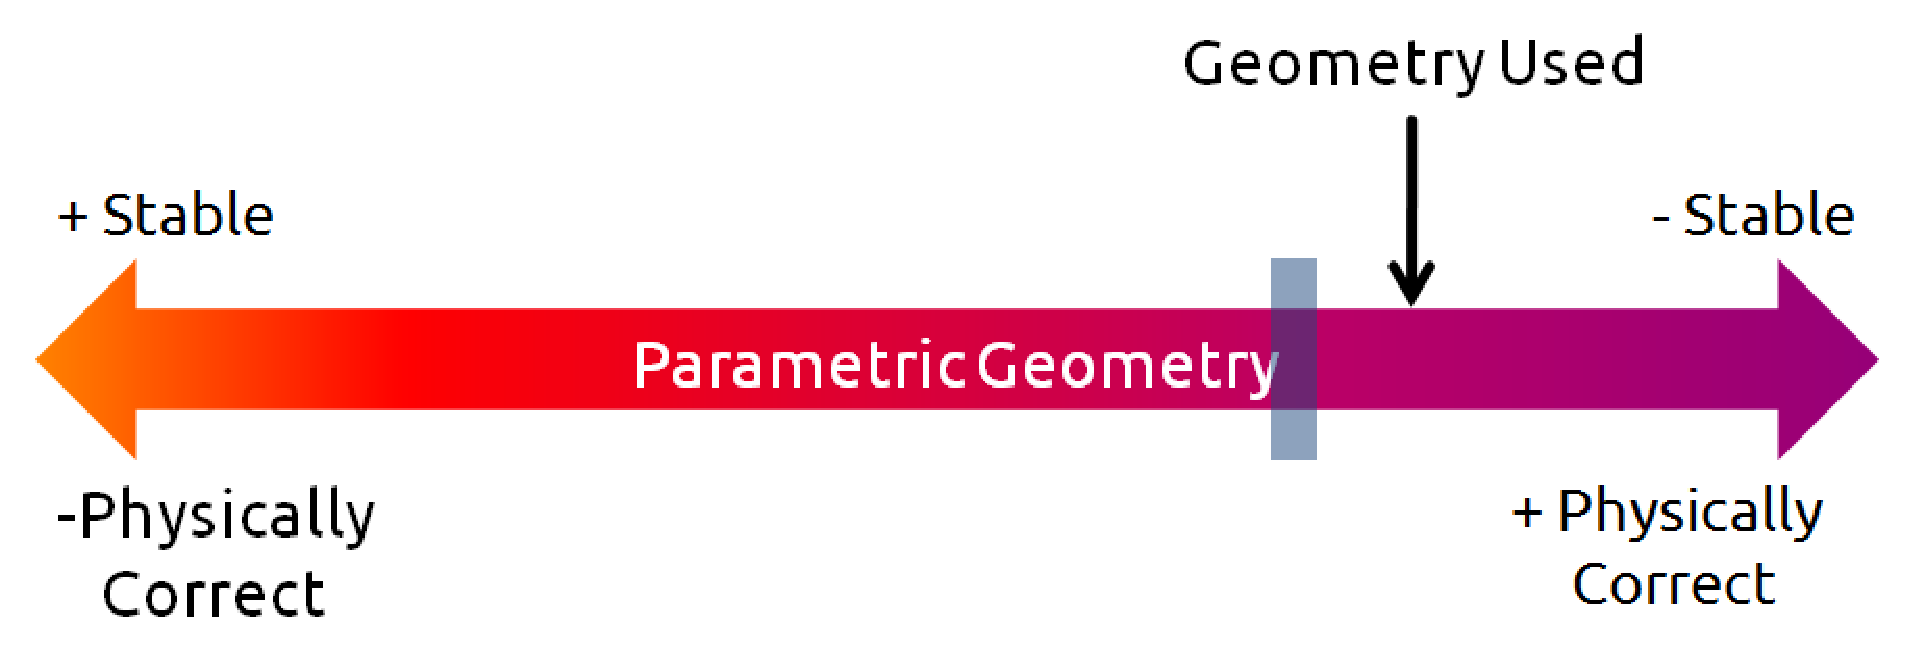
\includegraphics[width=9cm]{images/geometriaparametrica-translate.eps}
\caption{The proposed parametric geometry of the foot allows the user to
         balance stability and physical correctness of the simulation.}
\label{fig:EstabVsCorrFis}
\end{figure}

It is important to note that there may happen some cases more stable than those granted by the foot geometry indeed used in the simulation (i.e. the blue bar on the left side of the used geometry, as in Figure \ref{fig:EstabVsCorrFis}), where the generated motion can still be considered physically correct. In these situations, only the used geometry is not suitable for the desired motion.
However, if the used geometry is improved in a realistic manner, in order to increase stability, the previously acquired motion would be validated.
Therefore, we can say that the physical correctness of the motion is, in fact, independent of the used geometry.
%
Note also that, in the more unstable case, where no torque is artificially compensated (i.e. the blue bar on the rightmost side), the torque applied to the foot can still be compensated, regardless of the parametric geometry, by the interaction between the geometry of the foot indeed used in the simulation and the ground.
%Portanto, a geometria paramétrica é independente da geometria usada na simulação.

%
Before explaining in more details the used parametric geometry, it is important to realize that the idea of decoupling the geometry of the foot used in the simulation from its interaction with the ground introduces an abstract representation of this interaction. 
The concrete structure of this representation, which defines the meaning of the parameters, is not unique.
%A única exigência é que essa representação abstrata seja coerente em relação à compensação do torque aplicado no pé.
The only requirement is that there should be consistency in relation to the compensation of the torque applied to the foot.
After all, the defined structure and the choice of the parameters must determine how much torque applied to the foot should be compensated.
Furthermore, it is desired that the manipulation of these parameters be simple. %simples/fácil/intuitiva
Therefore, although it is necessary to define a specific structure, the contribution of using a detached abstract representation goes beyond the limits imposed by a chosen structure in particular. The structure chosen in this work is described below.


%\begin{figure}[h]%[!htbp]
%     \begin{center}
%     \includegraphics[height=3.5cm]{conefriccao.png}
%     %\caption{Cone de Fricção para um pé cilíndrico. (a) Vista superior. (b) Vista lateral.}
%     \caption{Modelagem de contato utilizada para o pé de apoio, baseada no cone de fricção de Coulomb. (a) Vista superior do pé. (b) Vista lateral do pé.}
%     \label{fig:conefriccao}
%     \end{center}
%\end{figure}

For simplicity, some restrictions on the used structure are defined.
First, the geometry chosen to represent the foot has a cylindrical shape, as illustrated in Figure \ref{fig:visaogeral}c (top and side views).
%Analisando
Assuming the illustrated form, one can predict the extreme situation where the maximum torque in the foot would be offset, namely, 
a resultant ground reaction force being applied to one end of the contact of the cylinder with the ground.
Due to the symmetry of the cylinder, without loss of generality, it can be assumed that this resultant force is applied to the rightmost end of the corresponding circle, which represents the contact area between the cylinder and the ground.
Based on \emph{Coulomb’s model of friction} positioned in this extreme contact point, it is also assumed that the resultant force capable of 
compensating the maximum torque on the foot is in accordance with the scheme illustrated in Figure \ref{fig:visaogeral}c, in which there is
a vector, $GRFmax$, located in the limit of the cone defined by the angle $\theta$. 
Whereas the foot has uniform density, it is still necessary to define the dimensions of the cylinder and a maximum length for the vector $GRFmax$.
Thus, one can calculate the maximum compensatable torque, $\tau_{comp}$, as:
%
\begin{equation}
  %\tau_{comp} = GRF_{max} \times D_{com} = \left( \begin{array}{c}  mcos\theta \\ msen\theta \\ 0 \end{array} \right) \times \left( \begin{array}{c}  -r \\ h \\ 0 \end{array} \right),
  \tau_{comp} = D_{com} \times GRF_{max}
              = \left( \begin{array}{c}  -r \\ h \\ 0 \end{array} \right) \times \left( \begin{array}{c}  m\mathrm{cos}\theta \\ m\mathrm{sin}\theta \\ 0 \end{array} \right),
\end{equation}
%
where $h$ is the distance from the ground to COM of the foot, $r$ is the foot's radius, $m$ is the length of the vector $GRFmax$ and $\theta$ is the angle of the friction cone.
%
It is important to emphasize that these four parameters are user defined.
And it is through the choice of values for these parameters that the user is capable of, abstractly, sliding the bar illustrated in Figure \ref{fig:EstabVsCorrFis}.

%$\tau_{comp}$ é sempre horizontal.
Considering all the mentioned assumptions, it is possible to verify a limitation on the chosen structure: $\tau_{comp}$ is always horizontal and, thus,
is not able to compensate for any vertical component of torque applied to the foot.
%Assume-se que o torque aplicado no pé em torno do eixo vertical é sempre totalmente compensado.
Again, for simplicity, it is assumed that the vertical component is always completely compensated, in an artificial way.
%
%módulo
Furthermore, again due to the symmetry of the cylinder, only the length of the maximum compensable torque is necessary in order to determine how much of the torque applied to the foot must be compensated.
For any direction of the torque applied to the foot, the extreme point of contact and direction of the vector $GRFmax$ can be conveniently adapted, getting always the same scheme of the Figure \ref{fig:visaogeral}c.

%A razão de compensação do torque aplicado ao pé é definida por:
Consider the following ratio, corresponding to the percentage of the torque applied to the foot which will be compensated:
%
\begin{equation}
 %ratio  = \frac{\| \tau_{comp} \|}{\| \tau_{foot}\bot \|}, %1\geqslant ratio>0,
 comp  = \frac{\| \tau_{comp} \|}{\| ^{foot}\tau_{bal}\bot \|}, %1\geqslant ratio>0,
\end{equation}
%
where $^{foot}\tau_{bal}\bot$ is the horizontal projection of the torque applied in the stance foot, extracted from the balance control (Equation \ref{eq:pd_eq}). %(Seção \ref{}). %projeção/componente
Note that $^{foot}\tau_{bal} = -^{ankle}\tau_{bal}$ and $\| \tau_{comp} \| = |$\textit{h} \textit{m} cos$\theta$ + \textit{r} \textit{m} sin$\theta$$|$.
%Caso $ratio > 1$, considerar $ratio = 1$. $0 \leq ratio \leq 1$.
%The value of $comp$ is in the range [0, 1]. If $comp$ is greater than 1, the value is truncated. %definido como igual a 1.
Once the value of $comp$ is truncated if it is greater than 1, %truncado = definido como igual a 1.
it will always be in the range [0, 1].
In Figure \ref{fig:EstabVsCorrFis}, increasing the value of $\| \tau_{comp} \|$ (and, consequently, of $comp$) corresponds to moving the slider to the left.
Therefore, the total torque applied to the support foot of the simulated character is defined according to this ratio of compensation:
%
\begin{equation}
  %^{foot}\tau_{total} = ^{foot}\tau_{pd} + ^{foot}\tau_{eq}*ratio.
  %^{foot}\tau_{total} = (^{foot}\tau_{pd} + ^{foot}\tau_{eq}\bot)*(1-ratio).
  ^{foot}\tau_{total} = ^{foot}\tau_{pd} + ^{foot}\tau_{bal}\bot (1-comp).
\end{equation}
%
%Diferente de um modelo de contato mais complexo, tal como o utilizado por \cite{bib:Jain11}, foi utilizado esse modelo mais
%simples que promove resultados desejados, quando comparados aos resultados da simulação seguindo os dados de referência.
%
%O usuário pode também especificar uma tolerância para a porcentagem do torque absorvido pelo pé. A estratégia de equilíbrio deve ser desativada caso a
%%Esse valor estipula que o personagem deve desativar a estratégia de equilíbrio caso a
%porcentagem do torque compensado ($ratio$) esteja abaixo do valor de tolerância.
%Isso serve para que o personagem possa cair mais naturalmente.
%%Este controle promovido pelo pé desacoplado do modelo simulado visa dar plenos poderes para o usuário determinar como a animação deve se comportar.
When this percentage ($comp$) of compensation is below a certain tolerance value chosen by the user, the balance control can be turned off, allowing the character to fall more naturally.
When turning it off, increasing the damping in PD controllers also helps to get a more natural fall.
%%%%%%%%%%%%%%%%%%%%%%%%%%%%%%%%%%%%%%%%%%%%%%%%%%%%%

%%%%%%%%%%%%%%%%%%%%%%%%%%%%%%%%%%%%%%%%%%%%
% Subseção a traduzir e editar o texto
\subsection{Sensor de Contato}

Neste trabalho são utilizadas duas metodologias para determinar qual o pé do personagem simulado que é considerado pé de apoio
para os cálculos da matriz Jacobiana. Uma é ativada quando o personagem não segue um movimento capturado e a outra é utilizada 
quando o mesmo é guiado para seguir um movimento capturado. Sendo assim, utilizamos dois tipos de sensores que funcionam de 
acordo com a metodologia utilizada. Para a primeira metodologia, o sensor leva em consideração a posição dos pés, suas GRFs e a 
projeção do COM do personagem no solo e no segundo caso considera-se o pé que se presume estar em contato com o solo do 
movimento capturado e as GRFs do personagem simulado. Em ambos os casos, a metodologia é realizada em cada instante da simulação.

\begin{figure}[!ht]
\centering
\def\svgwidth{\columnwidth}
\input{images/change_foot.pdf_tex}
\caption{Esquema da determinação do pé de apoio quando o personagem não segue um movimento capturado. Os raios das circunferências
         em vermelho (zona de influência) são determinados pelo usuário, cujo centro é o meio do pé do personagem. 
         Se a projeção do COM ($com\bot$) estiver dentro desta zona de influência do pé considera-se o contato deste pé com o solo (ficando verde)
         ou se $com\bot$ não estiver em nenhuma das duas zonas de influência. Caso a $com\bot$ não estiver em uma zona de influência
         e estiver na outra zona de influência o pé fica no ar (ficando azul).}
\label{fig:sensortroca}
\end{figure}

Quando o personagem não segue um movimento capturado ele independe de informações externas para determinar o contato com o solo,
sendo assim necessárias apenas informações que o próprio ambiente físico pode promover. Neste caso, as GRFs são ideais para se 
determinar o contato do pé do personagem com o solo, porém não é suficiente para determinar se o pé em contato será o pé de 
apoio (para fins de equilíbrio). Sendo assim utilizamos a seguinte metodologia para determinar o pé de apoio do personagem, de 
acordo com a Figura \ref{fig:sensortroca}. Quando a projeção do COM encontra-se em um dos círculos de influência e existe GRFs 
determinamos este pé como sendo um pé de apoio, ou se o COM não se encontrar em nenhuma das zonas de influência dos pés.

%O animador determina qual valor do módulo mínimo para a soma das GRFs do pé, com base neste valor, caso o pé não apresente
%um valor superior ao determinado este pé é desconsiderado no controle de equilíbrio e naturalmente desconecta-se
%do solo. Dessa forma, o personagem pode trocar as hierarquias de Jacobiana mesmo sem seguir um movimento capturado.



\begin{figure}[!ht]
\centering
\def\svgwidth{\columnwidth}
\input{images/foot-changevector.pdf_tex}
\caption{Quando a força de controle ($f_{c}$) e o vetor de direção do pé que encontra-se em apoio ao pé que está
         no ar ($d$), ambos projetados no solo, possuem a mesma direção, $f_{c}$ não será alterado. Caso
         contrário $f_{c}$ será projetado no vetor ${d}$, utilizando assim a força de controle paralela ($f_{c \parallel}$) ao vetor $d$, fazendo com que o pé que esteja no solo possa
         se tornar pé de apoio de forma mais natural.}
\label{fig:umpeparadois}
\end{figure}



No entanto faz-se necessária uma análise da mudança dos pés de apoio, de dois pés para um pé e de um pé para um dois pés. 
O primeiro caso é simples, basta verificar se o COM está projetado em uma única zona de influência para desligar o outro pé
como pé de apoio, no entanto o segundo caso para deixar a transição mais natural realizamos uma alteração na força de controle
(responsável por levar o COM para o ponto de equilíbrio desejado). Observa-se a Figura \ref{fig:umpeparadois}, no primeiro caso temos
que quando os vetores estão na mesma direção utilizamos a força de controle já calculada anteriormente (Equação \ref{eq:forcacontrole}),
caso contrário faremos uma decomposição para determinar a força de controle de modo que faça com que o COM se estabilize em
direção ao pé que está no ar de acordo com a seguinte equação:
\begin{equation}
  f_{control} = f_{control} - {d}_{u} (f_{control} \cdot {d}_{u}) 
\end{equation}
\noindent onde, ${d}_{u}$ é o vetor unitário determinado pela posição do pé de apoio ao pé que está no ar projetado no solo. 
Desta forma, a transição de um pé para dois pés fez com que o movimento parecesse mais natural.
Sendo assim, o personagem pode trocar as hierarquias de Jacobiana mesmo sem seguir um movimento capturado.



Ao trabalhar com movimentos de referência, observamos em alguns casos que nos movimentos com locomoção o personagem chega a ``arrastar'' o pé no chão mesmo quando ainda executa
um movimento, desta maneira não existe uma exatidão para determinar quando o pé deve considerar-se no ``ar'' ou apoiado no solo. 
Esses casos poderiam levar uma descontinuidade do movimento do pé no personagem simulado. Observando isso, o sensor utilizado para
determinar qual o pé que está apoiado, ao seguir um movimento de referência, leva-se em consideração dois quesitos: quando
o pé pode se desconectar do solo e quando o pé pode se conectar ao solo, ou seja, ser configurado como pé de apoio. No primeiro quesito é necessário somente as informações adquiridas do movimento
capturado, no segundo são utilizadas duas informações em conjunto, informações adquiridas do movimento de referência e das GRFs de contato do pé 
do personagem simulado. 


Os movimentos de referência não trazem consigo dados que determinam qual o pé que está em contato com o solo, para complementar esta carência
determinou-se manualmente uma estrutura que dita qual o pé que possa estar em contato, ou não, com o solo em cada \textit{frame} do movimento capturado.
Essa informação se faz necessária para se adquirir simulações mais comportadas de acordo com o movimento a ser seguido, vendo-se que a técnica
proposta necessita, para que seu controle funcione da melhor forma possível, da informação de que pé dever ser considerado de apoio. No caso do pé desconectar-se do solo 
utilizamos as informações dessa estrutura, caso o pé não seja considerado pé de apoio na estrutura, a fricção deste pé, no personagem simulado, é zerada
fazendo com que o pé deslize no solo, em algumas situações. Para determinar qual pé deve estar contato com o solo é verificado primeiramente se o pé na estrutura
está em contato com o solo, naquele determinado instante, caso esteja observa-se a soma das GRFs no eixo y, se for maior que zero o pé do
personagem é considerado pé de apoio. Caso um dos requisitos não seja verdadeiro o pé é não é considerado como pé de apoio na simulação.


Com base no controle de equilíbrio, simplificação de contato e no esquema de sensores elaborou-se uma série de testes e os resultados podem ser conferidos na seção seguinte.


\section{Results}

The experiments have used a humanoid character model with mass of approximately 72kg. Open Dynamics Engine (ODE) \cite{bib:ODE} has been used for the
simulation, with gravitational acceleration \textit{g}=-9,8$m/s^{2}$, friction coefficient $\mu$=1.0, and simulation step 0.0005s \cite{bib:Coros10}. Ground contact have been
simulated with \textit{Error Reduction Parameter} (ERP) and \textit{Constraint Force Mixing} (CFM) equals to ERF = 0.02 and CFM = 0.0001. A mesh has been used only
for rendering (Figure \ref{fig:modeloutilizado}b), and does not influence over the physical simulation at all. All simulations have been performed in real time on a 
2.20GHz x 8 Intel Core i7 machine.

In this work, the proposed balance strategy allows the character to follow captured motions or static poses, obeying some goals imposed by the
user. A series of experiments was performed to demonstrate some of the features and applications of the control structure. An accompanying video
is available for better visualization and evaluation of the results. In all tests, the simulated character has 13 spherical joints, totaling 39 
internal DOFs, and boxes are used as the geometries of all links (including the feet) (Figure \ref{fig:modeloutilizado}a). The video shows the character in different
situations, in both double and single stance, with two feet on the ground and with a single support foot.


\begin{figure}[tbh]
\centering
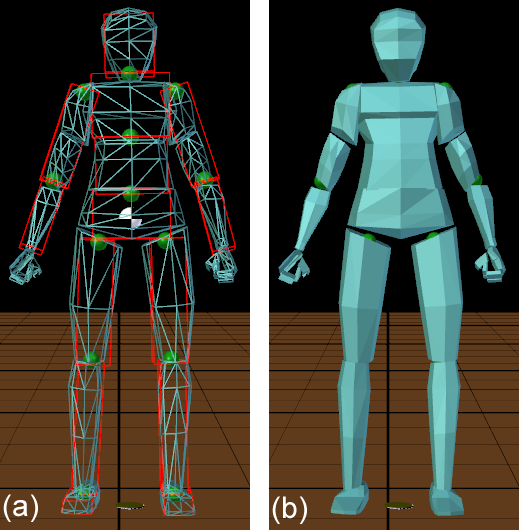
\includegraphics[width=5cm]{images/modelo-utilizado.png}
\caption{Character used in the tests. (a) The red wireframe corresponds to the shape
of the character’s links, as considered in the simulation. The green spheres represent the joints, which are all spherical.
(b) Character's mesh used only for rendering.}
\label{fig:modeloutilizado}
\end{figure}

%\noindent \textbf{Parâmetros dos controladores}.
\noindent \textbf{Virtual control terms}. The influence of each term of the virtual controller over balance has been tested: control force, gravity compensation,
linear momentum error, control torque and angular momentum error. These terms directly influence the character's balance and were based on other
works. As some examples, \cite{bib:Macchietto09} used angular momentum, \cite{bib:Geijtenbeek12} \cite{bib:Zordan02} used the goal of keeping 
the COM over the center of a support region, and \cite{bib:Coros10} used individual Jacobians to compensate gravity, though not in a unified
manner, as in this work.

%Somamos a isto a habilidade de todos os \textit{links} do personagem atenderem a uma orientação desejada no peito no termo torque de controle.
\noindent \textbf{Tracking captured motions}. To track reference motions, PD controllers were used in the joints. However, the goal of the PD
controllers may conflict with the goals of the balance control. In order to show that these two components of the controller adapt well while
tracking the captured motions, Figure \ref{fig:grafico-quadril-direito} shows the graphs of the angles (axis x, y and z) of the character's right hip as an example, comparing 
the captured and simulated motions. Note that, as in \cite{bib:Geijtenbeek12}, we can use the captured motion directly, without any adaptation to the control 
proposed in this paper.

%Assim, observamos que mesmo sendo aplicados torques internos a partir dos controladores PD e do controle de equilíbrio em cada junta do personagem,
%este consegue em geral executar o movimento desejado.
%

\begin{figure}[thbp]
\centering
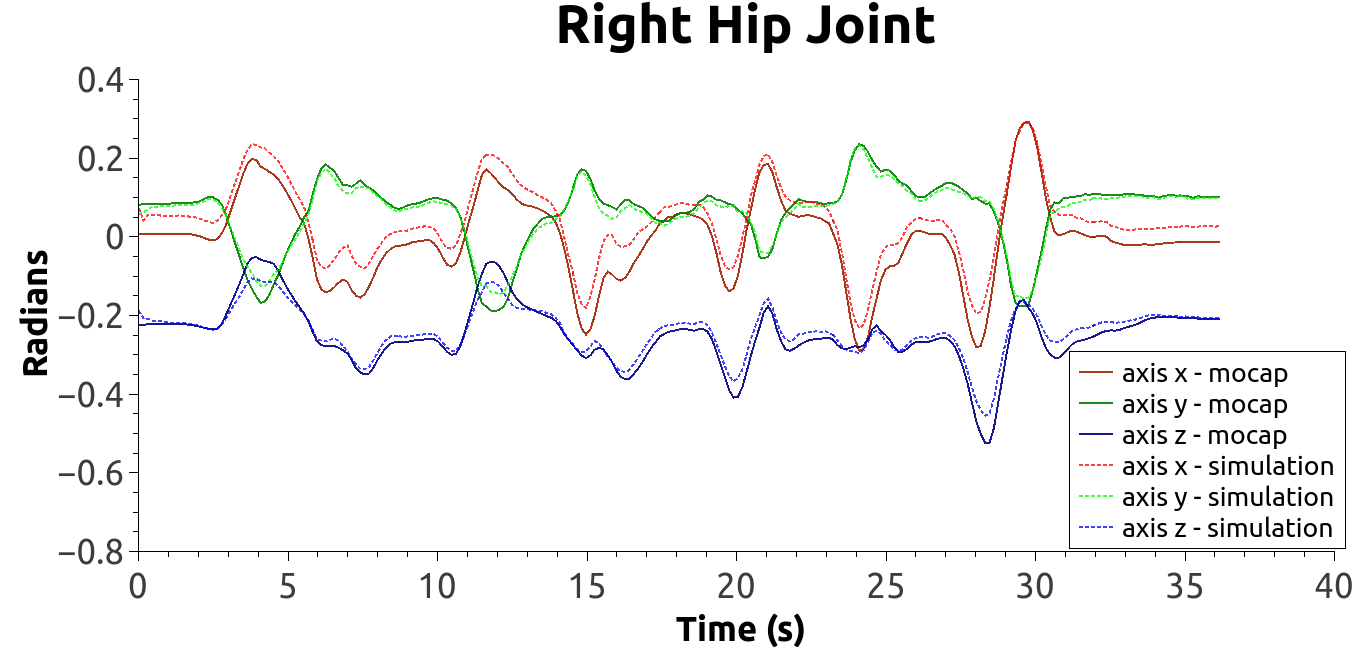
\includegraphics[width=9cm]{images/ombro-direito-translate.png}
\caption{Angular difference, at the right hip joint, between captured and simulated motions.
In the considered motion, the character is throwing punches (see the reference video).}
\label{fig:grafico-quadril-direito}
\end{figure}


\begin{figure}[!tbh]
     \centering
     \includegraphics[width=18.4cm]{images/filmstrip-pelvis.eps} %height=5cm,
     \caption{Response of the balance control in the presence of an external stimulus.
              Using all links of its body, as a whole, the character automatically keeps the center of mass (black and white ball)
              over the support area while its pelvis is moved by an external controller.}
     \label{fig:controle-externo}
     \centering
\end{figure}

\noindent \textbf{External disturbances}. In performed tests, the character was disturbed in two ways: through external forces directly applied
and through collisions with objects thrown at him. External forces were applied in standing position, focusing on the overall motion of all links
working together in the balance recovery. The objects were thrown on random parts of the character, in order to observe its behavior while
tracking captured motions. The thrown objects were spheres with density of 100$kg/m^{3}$ and velocity varying between 7$m/s$ and 15$m/s$. The density was gradually increased to the point that the character could not remain standing (approximately in the density of 125$kg/m^{3}$).

%Foram realizadas colisões de esferas com o personagem em movimentos em um único pé de apoio e com os dois pés de apoio. O personagem manteve-se 
%em equilíbrio seguindo os movimentos capturados mesmo com estas perturbações externas.
\noindent \textbf{External controllers}. In order to observe further the influence of all links of the character to maintain balance, 
an external positional controller (Equation \ref{eq:pdforca}) was used. This controller operates at each instant of the simulation by applying an 
external force on a given link of the character so that the COM of this link reaches a virtual point, chosen by the user. The stability 
provided by the simplified contact allows the animator to easily tune the constants of the PD controllers, of the balance control and of 
these external controllers, according to his purpose. The Figure 6 shows an example in which the animator activates one of these external
controllers in order to move the pelvis of the character to front. Note that the balance control overlaps, clearly causing the character 
to be worked as a whole to keep the COM over the support region. The external force applied by the external positional control has the
following expression:

\begin{equation}
 f_{externa} = pks (pv - efetor) - pkd (\omega_{link}),
 \label{eq:pdforca}
\end{equation}
%
where $pv$ is the position of the virtual point informed by the animator, $effector$ is the current position of the COM of the link of the
character which must reach the $pv$, $\omega_{link}$ is the linear velocity of this link, and $pks$ and $pkd$ are user-chosen constants.

\noindent \textbf{Holding cup}. The animator can also restrict the orientations of character's specific links. In this test, an extra internal
PD controller was used at the character's wrist in order to restrict, in global coordinates, the link that represents its hand. Note that only
the rotations in the x and z axes are controlled so that they do not turn the cup (cup is free to rotate on the y axis). It was observed that 
the character could both track captured motions and balance itself while still respecting this additional constraint (see the reference video).



%Para o personagem seguindo o movimento de balançar a perna com um único pé de apoio segurando uma xícara e apoiado com os dois pés segurando duas xícaras enquanto 
%a pélvis é puxada por meio de um controlador externo a robustez do controlador de equilíbrio foi alcançada.

%\textbf{Contato Simplificado}. A principal contribuição deste trabalho é a concepção de uma estrutura desvinculada da estrutura simulada para
%o pé do personagem a fim de simular um pé mais real. Esta estrutura de contato simplificado busca uma estabilidade para o controle de equilíbrio, 
%governada pela compensação do torque aplicado do tornozelo ao pé do personagem que por sua vez irá interagir com o solo. Sem esta compensação 
%o personagem fica suscetível a instabilidades. Como foi evidenciado na inicialização do personagem, no qual ele não consegue manter-se em pé sem
%o contato simplificado. Depois de inicializado, o personagem é capaz de manter-se em pé mesmo sem a estrutura de contato simplificado. No entanto, 
%com pouca intervenção externa o equilíbrio deixa de ser um objetivo alcançável, não mantendo-se em pé, mostrando assim que o contato simplificado
%promove bons resultados que podem ser observados nos testes discutidos a seguir.

\noindent \textbf{Simplified contact}. Some tests were performed in order to specifically verify the contribution of using the proposed simplified
contact model (see the reference video). The first test shows that the initialization of the simulation is greatly facilitated. Without the 
proposed model, the animator would need to finely adjust the initial pose of the character or use optimization, as in \cite{bib:Geijtenbeek12}. 
Moreover, soon after it is initialized, the character becomes stable enough to balance itself even without the simplified contact. The second 
test compares the character’s behavior under external intervention of the environment, with and without using the simplified contact, testifying
the stability provided by the proposed simplification again. The third test shows that, if preferable, it is still allowed to the animator to 
sacrifice a bit of physical correctness of the simulation in exchange for even greater stability, by just adjusting the parameters of the
simplified contact.
%%%%%%%%%%%%%%%%%%%%%%%%%%%%%%%%%%%%%%%%%%%%%%%%%%%%%

\section{Discussion and Future Work}

%Practical appeal
The ease of playing captured motions directly, without worrying about the stability of a character, is clearly a huge draw for animators that 
produce games, movies and virtual environments in general. However, the treatment of balance is one of the main difficulties when trying to add 
physics to the environment and, of course, to the characters. The requirement of additional knowledge, often involving complicated issues to deal
with, such as when using optimization, greatly discourages the use of physics, especially for novice animators. We believe that the convenience
provided by our simplified contact model is the main contribution of this work. The ensured stability and the ease with which the torque
compensation on the supporting foot is implemented should shorten the transition from the approaches that produce purely cinematic animation to
those that produce physically based animation. Thus, this paper aims at helping animators to migrate from purely cinematic approaches to dynamic
approaches.

%Optimization - using in future work
It is fair to say that, although the proposed approach has a useful practical appeal, trying to simulate accurately the morphology of animals in
general (not just humans) is still essential, and obviously deserves a lot of research. In this sense, optimization has proven to be very useful 
\cite{bib:Nunes12} \cite{bib:Geijtenbeek12} \cite{bib:Wang12} \cite{bib:Geijtenbeek13}. For future work, we believe that the proposed model can
be used to improve the search space based on the work of \cite{bib:Panne95}, but more effectively. The idea would be to minimize the artificial 
compensation torque on the supporting foot, and to get an optimized result that works without the simplified contact. In other words, if the 
objective function is well behaved because of the stability provided by the simplified contact, the optimizer would be directed to a shorter 
and safer path (with less local minima) to achieve the final result.

%Otimização - usar em trabalhos futuros
%Moreover, although the proposed method has a useful practical appeal make efforts to accurately simulate the morphology of animals in general
%(not just humans) is still essential, and obviously deserves a lot of research. %esforço de pesquisa.
%In this sense, optimization has proven increasingly useful \cite{bib:Nunes12} \cite{bib:Geijtenbeek12} \cite{bib:Wang12} \cite{bib:Geijtenbeek13}. %útil/necessária
%For future work, it is believed that the proposed model can be used to improve the performance of the search space based on the work of \cite{bib:Panne95}
%but more significantly.
%The idea would be to minimize the artificial compensation torque on the supporting foot and get a final result of the optimization that works without the simplified contact.
%In other words, once the optimization function would be better behaved because of the stability provided by the simplified contact, the optimizer would be directed
%for safer path (with less local minima) and shorter to achieve the final result.
%%%%%%%%%%%%%%%%%%%%%%%%%%%%%%%%%%%%%%%%%%%%%%%%%%%%%

% conference papers do not normally have an appendix
\newpage

\appendix

%--------------------------------------------------------------------------------------------------------

\subsection{Spatial Vector Notation}\label{ap:notacao6D}

The \textit{spatial vector notation} is based on \cite{bib:Cline99,bib:NunesTese12},
and is used throughout the formulation related to the Jacobian.
Basically, this notation consists in concatenating angular and linear information in vectors with six coordinates.
The main advantage is that such grouped information may be transformed between different coordinate frames in an unified way,
by using the \textit{adjoint matrices}.

A \textit{spatial velocity}, also known as \emph{twist}, is represented by the vector $\phi = (\omega^T ~ v^T)^T$,
where $\omega$ corresponds to an angular velocity and $v$ corresponds to a linear velocity.
Similarly, a \textit{spatial force}, also known as \emph{wrench}, is represented by the vector
$w = (\tau^T ~ f^T)^T$, where $\tau$ corresponds to a torque and $f$ corresponds to a force.
%Nao ficou legal mostrar vetores 6D na vertical: \left( \begin{array}{cc} \omega \\ v \end{array} \right)

The adjoint matrix, $^{b}_{a}Ad$, with dimension 6$\times$6, transforms a spatial velocity, $^a\phi$, given in coordinates of $a$,
at a corresponding spatial velocity, $^b\phi$, given in coordinates of $b$: $^b\phi = {^{b}_{a}Ad} ~ ^a\phi$.
$^{b}_{a}Ad$ can be easily constructed from the corresponding \textit{homogeneous transformation matrix} $^{b}_{a}T$:
%
\begin{equation}
 %\left( \begin{array}{c} ^{w}\omega \\ ^{w}v \end{array} \right) = _{i}^{w}Ad \left( \begin{array}{c} ^{i} \omega \\ ^{i} v \end{array} \right)
 %\quad \mathrm{, onde}\quad
 ^{b}_{a} T = \left[ \begin{array}{cc} R & p \\   0  & 1 \end{array} \right], \quad
 ^{b}_{a}Ad = \left[ \begin{array}{cc} R & 0 \\ \left[p\right]R & R \end{array} \right],
\end{equation}
%
where $[p]$ corresponds to the skew-symmetric matrix, with dimension 3$\times$3, equivalent to the cross product $p\times$:
%
\begin{equation}
 [p] = p\times = \left[ \begin{array}{ccc} 0 & -p_{z} & p_{y} \\ p_{z} & 0 & -p_{x} \\ -p_{y} & p_{x} & 0  \end{array} \right],
\end{equation}
%
where $p_{x}$, $p_{y}$ and $p_{z}$ are the coordinates of the vector $p$.
%
Note that the inverse transpose of $^{b}_{a}Ad$ transforms \emph{spatial forces}: $^{b}w = {^{b}_{a}Ad^{-T}} ~ ^{a}w$. %, onde $w$ representa uma força 6D.
Namely, its transpose transforms \emph{spatial forces} of $b$ to $a$: $^{a}w = {^{b}_{a}Ad^{T}} ~ ^{b}w$.
%Note que $w = {\left( \begin{array}{c} \tau \\ f \end{array}  \right)}$, onde $\tau$ corresponde a um torque e $f$ corresponde a uma força.

%$\prescript{b}{a}{M}$ corresponde a uma matriz de massa, escrita em notação 6D (de dimensão 6$\time$6), que agrupa inércia $\mathcal{I}_a$ e massa $m_a$, em coordenadas de b:
The mass of a given system $a$ may also be defined using the spatial vector notation. A matrix with dimension 6$\times$6 is used to group its inertia $\mathcal{I}_a$ and its mass $m_a$:
%
\begin{equation}
  \prescript{b}{a}{M} = \left[ \begin{array}{cc} {^b\mathcal{I}_a} & 0 \\ 0 & m_{a} I \end{array} \right],
  \label{eq:inerciamassa}
\end{equation}
%
where $\prescript{b}{a}{M}$ is the \emph{spatial mass} of $a$ in the coordinates of $b$, and $I$ is the identity matrix with dimension 3$\times$3.




%\section{Citations and References}

%\subsection{Citations}

%The SIGGRAPH citation format is the ``author year''
%format~\cite{Pellacini:2005:LAH}. The year is separated from the
%author by a single space~\cite{yee:2000:ssa}. Two authors are
%separated by the word ``and''~\cite{parke:1996:CFA}. More than two
%authors are represented by the primary author and ``et al.''~\cite{levoy:2000:TDM}.

%Multiple citations at a single point in the content are separated by
%semicolons~\cite{levoy:2000:TDM,sako:2001:SSB}.%

%When the last name of the cited author is part of the text, it may be
%omitted from the citation: ``\ldots as shown in Fedkiw et
%al.~\shortcite{fedkiw:2001:VSO}, the coefficient remains\ldots''

\bibliographystyle{acmsiggraph}
%\nocite{*}
\bibliography{template}
\end{document}
